% Define document class
\documentclass[twocolumn]{aastex631}

% Filler text
\usepackage{blindtext}

% Begin!
\begin{document}

% Title
\title{An open source scientific article}

% Author list
\author{First Author}

% Abstract with filler text
\begin{abstract}
    \blindtext
\end{abstract}

% Main body
\section{Introduction}

\begin{figure}[ht!]
    \begin{centering}
        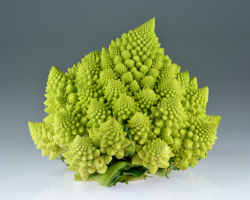
\includegraphics[width=0.4\linewidth]{static/broccoli.pdf}
        \caption{
            A static figure with a custom link, provided using the
            \texttt{marginicon} command within the \texttt{figure}
            environment.
        }
        \marginicon{\href{https://github.com}{\color{pink}\faGrinStars}}
        \label{fig:broccoli}
    \end{centering}
\end{figure}

\begin{figure}[ht!]
    \begin{centering}
        \includegraphics[width=0.4\linewidth]{figures/mandelbrot.pdf}
        \caption{
            An auto-generated figure with an auto-generated margin icon.
        }
        \label{fig:mandelbrot}
    \end{centering}
\end{figure}

\begin{figure}[ht!]
    \begin{centering}
        \includegraphics[width=0.4\linewidth]{figures/mandelbrot_light.pdf}
        \caption{
            An auto-generated figure with two vertically-stacked custom links.
            Any calls to the \texttt{marginicon} command supersede the auto-generated icons.
        }
        \marginicon{%
            \stackon[3pt]{%
                \href{https://github.com}{\color{blue}\faCat}%
            }{%
                \href{https://github.com}{\color{red}\faDog}%
            }%
        }
        \label{fig:mandelbrot_light}
    \end{centering}
\end{figure}

\end{document}
